%% Topology of ternary complex dimer identical
%% FigS3H4Tree.tex
%% Unused packages and definitions removed; TikZ/PGFPlots source formatted.

\documentclass[tikz,margin=2mm]{standalone}

\usepackage{amsfonts}
\usetikzlibrary{arrows}

\def \half {\frac{1}{2}}

\def\b{\mathsf{b}}
\def\c{\mathsf{c}}
\def\d{\mathsf{d}}

\begin{document}

\tikzstyle{every node}=[fill=white,rectangle,rounded corners,inner sep=1,outer sep=0]
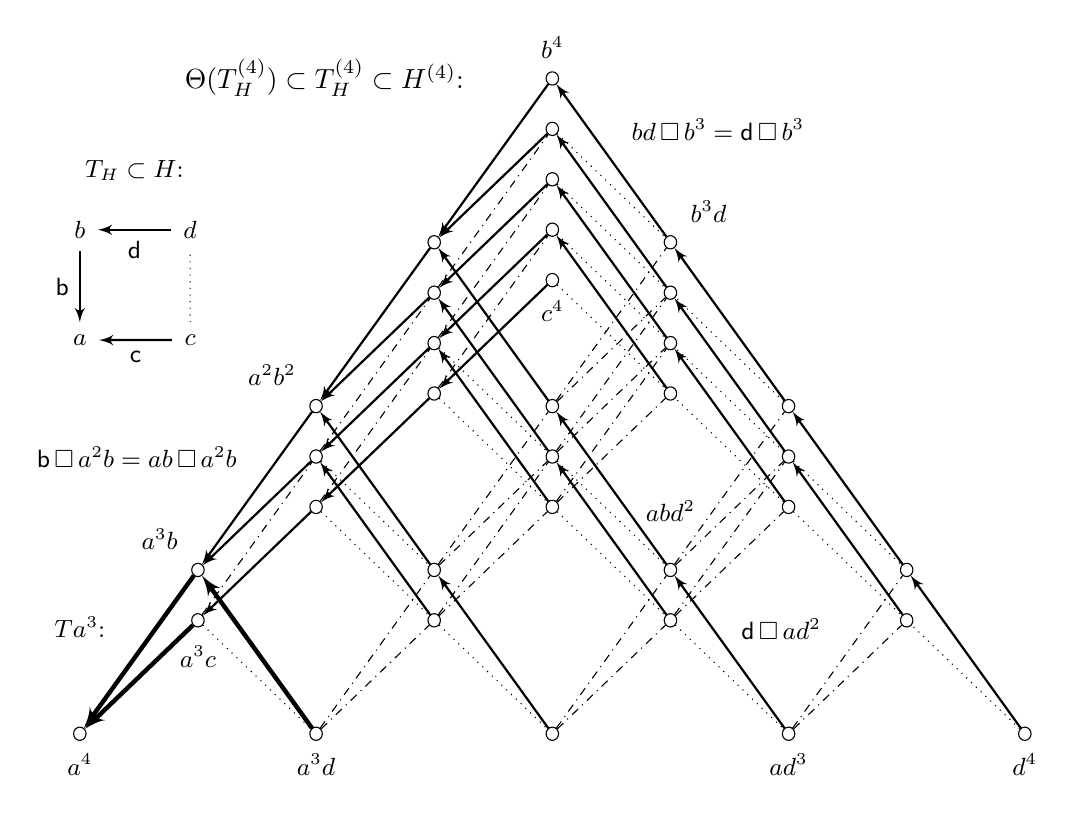
\begin{tikzpicture}[xscale=1.5,yscale=1.6,font=\small,shorten <=2.5pt,shorten >=2.5pt,>=latex']
    \def\rx{1}
    \def\ry{1.3}
    \begin{scope}
        \coordinate (a4) at (0*\rx,0*\ry);
        \coordinate (a3b) at (1*\rx,1*\ry);
        \coordinate (a2b2) at (2*\rx,2*\ry);
        \coordinate (ab3) at (3*\rx,3*\ry);
        \coordinate (b4) at (4*\rx,4*\ry);
        \coordinate (a3d) at (2*\rx,0*\ry);
        \coordinate (a2bd) at (3*\rx,1*\ry);
        \coordinate (ab2d) at (4*\rx,2*\ry);
        \coordinate (b3d) at (5*\rx,3*\ry);
        \coordinate (a2d2) at (4*\rx,0*\ry);
        \coordinate (abd2) at (5*\rx,1*\ry);
        \coordinate (b2d2) at (6*\rx,2*\ry);
        \coordinate (ad3) at (6*\rx,0*\ry);
        \coordinate (bd3) at (7*\rx,1*\ry);
        \coordinate (d4) at (8*\rx,0*\ry);
        \begin{scope}[yshift=-0.4cm]
            \coordinate (a3c) at (1*\rx,1*\ry);
            \coordinate (a2bc) at (2*\rx,2*\ry);
            \coordinate (ab2c) at (3*\rx,3*\ry);
            \coordinate (b3c) at (4*\rx,4*\ry);
            \coordinate (a2cd) at (3*\rx,1*\ry);
            \coordinate (abcd) at (4*\rx,2*\ry);
            \coordinate (b2cd) at (5*\rx,3*\ry);
            \coordinate (acd2) at (5*\rx,1*\ry);
            \coordinate (bcd2) at (6*\rx,2*\ry);
            \coordinate (cd3) at (7*\rx,1*\ry);
        \end{scope}
        \begin{scope}[yshift=-0.8cm]
            \coordinate (a2c2) at (2*\rx,2*\ry);
            \coordinate (abc2) at (3*\rx,3*\ry);
            \coordinate (b2c2) at (4*\rx,4*\ry);
            \coordinate (ac2d) at (4*\rx,2*\ry);
            \coordinate (bc2d) at (5*\rx,3*\ry);
            \coordinate (c2d2) at (6*\rx,2*\ry);
        \end{scope}
        \begin{scope}[yshift=-1.2cm]
            \coordinate (ac3) at (3*\rx,3*\ry);
            \coordinate (bc3) at (4*\rx,4*\ry);
            \coordinate (c3d) at (5*\rx,3*\ry);
        \end{scope}
        \begin{scope}[yshift=-1.6cm]
            \coordinate (c4) at (4*\rx,4*\ry);
        \end{scope}

        \node[above of=a4,yshift=10pt,xshift=0pt] {$Ta^3$:};

        \draw[<-,ultra thick] (a4) node[below,anchor=north,outer sep=4pt] {$a^4$} to (a3b);
        \draw[<-,thick] (a3b) node[above left,anchor=south east,outer sep=4pt] {$a^3b$} to node[above left,anchor=south east,outer sep=4pt] {$\b \, \Box \, a^2b  = ab \, \Box \, a^2b $} (a2b2) node[above left,anchor=south east,outer sep=4pt] {$a^2b^2$};
        \draw[<-,thick] (a2b2) to (ab3);
        \draw[<-,thick] (ab3) to (b4);

        \draw[dashdotted] (a3d) to (a2bd);
        \draw[dashdotted] (a2bd) to (ab2d);
        \draw[dashdotted] (ab2d) to (b3d);

        \draw[dashdotted] (a2d2) to (abd2);
        \draw[dashdotted] (abd2) to (b2d2);

        \draw[dashdotted] (ad3) to (bd3);

        %\draw[<-,thick] (b4) node[above,anchor=south,outer sep=4pt] {$b^4$} to node[above right,anchor=south west,outer sep=4pt] {$\frac{4}{3}\kappad[b^3] =\frac{4}{3}\kappad \eta_{\b\b\b\d} $} (b3d) node[above right,anchor=south west,outer sep=4pt] {$b^3d$};
        \draw[<-,thick] (b4) node[above,anchor=south,outer sep=4pt] {$b^4$} to node[above right,anchor=south west,outer sep=4pt] {$bd \, \Box \, b^3   = \d \, \Box \, b^3  $} (b3d) node[above right,anchor=south west,outer sep=4pt] {$b^3d$};
        \draw[<-,thick] (b3d) to (b2d2);
        \draw[<-,thick] (b2d2) to (bd3);
        \draw[<-,thick] (bd3) to (d4);

        \draw[<-,thick] (ab3) to (ab2d);
        \draw[<-,thick] (ab2d) to (abd2);
        \draw[<-,thick] (abd2) node[above,yshift=10pt,anchor=south,outer sep=4pt] {$abd^2$} to node[above right,anchor=south west,outer sep=1pt] {$\d \, \Box \, ad^2 $} (ad3) node[below,anchor=north,outer sep=4pt] {$ad^3$};

        \draw[<-,thick] (a2b2) to (a2bd);
        \draw[<-,thick] (a2bd) to (a2d2);

        \draw[<-,ultra thick] (a3b) to (a3d) node[below,anchor=north,outer sep=4pt] {$a^3d$};

        %% shift bc

        \draw[dashdotted] (a3c) to (a2bc);
        \draw[dashdotted] (a2bc) to (ab2c);
        \draw[dashdotted] (ab2c) to (b3c);

        \draw[dashdotted] (a2cd) to (abcd);
        \draw[dashdotted] (abcd) to (b2cd);

        \draw[dashdotted] (acd2) to (bcd2);

        \draw[<-,thick] (b3c) to (b2cd);
        \draw[<-,thick] (b2cd) to (bcd2);
        \draw[<-,thick] (bcd2) to (cd3);

        \draw[<-,thick] (ab2c) to (abcd);
        \draw[<-,thick] (abcd) to (acd2);

        \draw[<-,thick] (a2bc) to (a2cd);

        %% shift bc

        \draw[dashdotted] (a2c2) to (abc2);
        \draw[dashdotted] (abc2) to (b2c2);

        \draw[dashdotted] (ac2d) to (bc2d);

        \draw[<-,thick] (b2c2) to (bc2d);
        \draw[<-,thick] (bc2d) to (c2d2);

        \draw[<-,thick] (abc2) to (ac2d);

        %% shift bc

        \draw[dashdotted] (ac3) to (bc3);
        \draw[<-,thick] (bc3) to (c3d);

        %%%%

        \draw[<-,thick] (ab3) to (b3c);
        \draw[thin,dotted] (b3c) to (b3d);

        \draw[<-,thick] (ab2c) to (b2c2);
        \draw[thin,dotted] (b2c2) to (b2cd);
        \draw[<-,thick] (a2b2) to  (ab2c);
        \draw[thin,dotted] (b2d2) to (b2cd);

        \draw[<-,thick] (abc2) to (bc3);
        \draw[thin,dotted] (bc3) to (bc2d);
        \draw[<-,thick] (a2bc) to (abc2);
        \draw[thin,dotted] (bcd2) to (bc2d);
        \draw[<-,thick] (a3b) to (a2bc);
        \draw[thin,dotted] (bcd2) to (bd3);

        \draw[<-,thick] (ac3) to (c4);
        \draw[thin,dotted] (c4) to (c3d);
        \draw[<-,thick] (a2c2) to (ac3);
        \draw[thin,dotted] (c2d2) to (c3d);
        \draw[<-,thick] (a3c) to (a2c2);
        \draw[thin,dotted] (c2d2) to (cd3);
        \draw[<-,ultra thick] (a4) to (a3c) node[below,anchor=north,outer sep=4pt,yshift=-2pt] {$a^3c$};
        \draw[thin,dotted] (d4) to (cd3);

        \draw[dashdotted] (a3d) to (a2cd);
        \draw[dashdotted] (a2cd) to (ac2d);
        \draw[dashdotted] (ac2d) to (c3d);

        \draw[dashdotted] (a2d2) to (acd2);
        \draw[dashdotted] (acd2) to (c2d2);

        \draw[dashdotted] (ad3) to (cd3);

        \draw[thin,dotted] (a3c) to (a3d);

        \draw[thin,dotted] (a2c2) to (a2cd);
        \draw[thin,dotted] (a2cd) to (a2d2);

        \draw[thin,dotted] (ac3) to (ac2d);
        \draw[thin,dotted] (ac2d) to (acd2);

        \draw[thin,dotted] (a2bc) to (a2bd);

        \draw[thin,dotted] (abc2) to (abcd);
        \draw[thin,dotted] (abcd) to (abd2);

        \draw[thin,dotted] (acd2) to (ad3);

        \draw[dashdotted] (abd2) to (bcd2);

        \draw[dashdotted] (a2bd) to (abcd);
        \draw[dashdotted] (abcd) to (bc2d);

        \draw[dashdotted] (ab2d) to (b2cd);

        \def\vr{1.5pt} % \vr = vertex radius;  Set \vr = 2/scale for uniform sizing of vertices

        \draw[fill=white] (a4) circle(\vr);
        \draw[fill=white] (a3b) circle(\vr);
        \draw[fill=white] (a2b2) circle(\vr);
        \draw[fill=white] (ab3) circle(\vr);
        \draw[fill=white] (a3d) circle(\vr);
        \draw[fill=white] (a2bd) circle(\vr);
        \draw[fill=white] (ab2d) circle(\vr);
        \draw[fill=white] (b3d) circle(\vr);
        \draw[fill=white] (a2d2) circle(\vr);
        \draw[fill=white] (b2d2) circle(\vr);
        \draw[fill=white] (ad3) circle(\vr);
        \draw[fill=white] (bd3) circle(\vr);
        \draw[fill=white] (d4) circle(\vr) node[below,anchor=north,outer sep=4pt] {$d^4$};
        \draw[fill=white] (a3c) circle(\vr);
        \draw[fill=white] (a2bc) circle(\vr);
        \draw[fill=white] (ab2c) circle(\vr);
        \draw[fill=white] (b3c) circle(\vr);
        \draw[fill=white] (a2cd) circle(\vr);
        \draw[fill=white] (abcd) circle(\vr);
        \draw[fill=white] (b2cd) circle(\vr);
        \draw[fill=white] (acd2) circle(\vr);
        \draw[fill=white] (bcd2) circle(\vr);
        \draw[fill=white] (cd3) circle(\vr);
        \draw[fill=white] (a2c2) circle(\vr);
        \draw[fill=white] (abc2) circle(\vr);
        \draw[fill=white] (b2c2) circle(\vr);
        \draw[fill=white] (ac2d) circle(\vr);
        \draw[fill=white] (bc2d) circle(\vr);
        \draw[fill=white] (c2d2) circle(\vr);
        \draw[fill=white] (ac3) circle(\vr);
        \draw[fill=white] (bc3) circle(\vr);
        \draw[fill=white] (c3d) circle(\vr);
        \draw[fill=white] (c4) circle(\vr) node[below,anchor=north,outer sep=4pt] {$c^4$};
        \draw[fill=white] (b4) circle(\vr);
        \draw[fill=white] (abd2) circle(\vr);

        \node[left of=b4,yshift=-10pt,anchor=south east,fill=none,rectangle,font=\normalsize] {$\Theta(T_H^{(4)}) \subset T_H^{(4)} \subset H^{(4)}$:};

    \end{scope}

    \begin{scope}[xshift=0cm,yshift=4cm,node distance=1.4cm,>=latex',shorten <=1pt,shorten >=1pt]
        \node (B) {$b$};
        \node[below of=B] (A) {$a$};
        \draw[->,thick] (B) to node[left,align=center,inner sep=2pt,outer sep=2pt] {$\b$} (A);
        \node[right of=A] (C) {$c$};
        \draw[<-,thick] (A) to node[below,inner sep=2pt,outer sep=2pt] {$\c$} (C);
        \node[right of=B] (D) {$d$};
        \draw[->,thick] (D) to node[below,inner sep=2pt,outer sep=2pt] {$\d$} (B);
        \draw[dotted,thin] (C) to (D);
        \path (B) to node[above,yshift=0.5cm] {$T_H \subset H $:} (D);
    \end{scope}

    %\begin{scope}[xshift=0cm,yshift=4cm,node distance=1.3cm,>=latex',shorten <=0pt,shorten >=0pt,inner sep=1pt,outer sep=1pt]
        %\node (LRA) {$b$};
        %\node[below of = LRA] (RA) {$a$};
        %\draw [->,thick] (LRA) to  (RA);
        %\node[right of = RA] (RAG) {$c$};
        %\draw [<-,thick] (RA) to (RAG);
        %\node[right of = LRA] (LRAG) {$d$};
        %\draw [->,thick] (LRAG) to node[above,anchor=south,outer sep=4pt] {$T \subset H$}  (LRA);
        %\draw [dotted,thin] (RAG) to (LRAG);
        %\path (LRA) to  (LRAG);
        %\end{scope}
\end{tikzpicture}

\end{document}

